\chapter{Data Analysis}

\section{Example Table}

Table~\ref{tab:results} compares two models. The values are illustrative.

\begin{table}[htbp]
  \caption{Sample Quantitative Results}
  \label{tab:results}
  \begin{tabular}{lccc}
    \toprule
    Model    & Precision & Recall & F1-score \\
    \midrule
    Baseline & 0.78 & 0.74 & 0.76 \\
    Proposed & 0.85 & 0.83 & 0.84 \\
    \bottomrule
  \end{tabular}
  \tablenote{Higher values indicate better predictive performance.}
\end{table}

The proposed model has higher scores on all three measures.

\section{Example Figure}

Figure~\ref{fig:accuracy} shows illustrative validation accuracy over five
training stages.

\begin{figure}[htbp]
  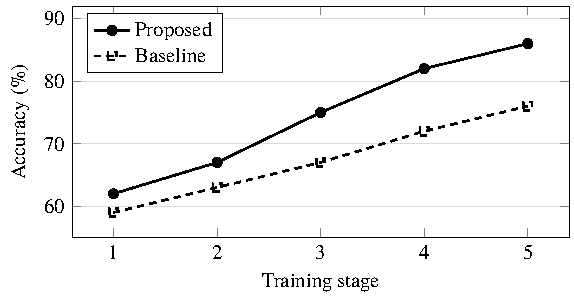
\includegraphics[width=0.7\textwidth]{figures/accuracy}
  \caption{Validation Accuracy by Training Stage}
  \label{fig:accuracy}
  \figuresource{Illustrative data.}
\end{figure}

The proposed model has higher accuracy at every stage.
